%%%%%%%%%%%%%%%%%%%%%%%%%%%%%%%%%%%%%%%%%%%%%%%%%%%%%%%%%%%%%%%%%%%%%%%%%%%%%%%%
% Author : Samuel Márton, Tomas Polasek (template)
% Description : Seventh exercise in the Introduction to Game Development course.
%   It deals with the creation of a Game Design Document, presenting a short 
%   pitch for a potential game project.
%%%%%%%%%%%%%%%%%%%%%%%%%%%%%%%%%%%%%%%%%%%%%%%%%%%%%%%%%%%%%%%%%%%%%%%%%%%%%%%%

\documentclass[a4paper,10pt,english]{article}

\usepackage[left=2.50cm,right=2.50cm,top=1.50cm,bottom=2.50cm]{geometry}
\usepackage[utf8]{inputenc}

% Hyper-Text References
\usepackage{hyperref}
\hypersetup{colorlinks=true, urlcolor=blue}

% Drawing Images and Graphs
\usepackage{tikz}
\usepackage{pgfplots}

% Page Utilities
\usepackage{graphicx}

% Image Sub-Captions
\usepackage{subcaption}

\newcommand{\ph}[1]{\textit{[#1]}}

\title{%
Game Pitch Document%
}
\author{%
Samuel Márton (xmarto03)%
}
\date{23/12/2023}

\begin{document}

\maketitle
\thispagestyle{empty}

{%
\large

\begin{itemize}

\item[] \textbf{Title:} \textit{Solitaire: Battle Royale}

\item[] \textbf{Genre:} \textit{Combat card game}

\item[] \textbf{Style:} \textit{2D retro pixel art}

\item[] \textbf{Platform:} \textit{Windows and Linux initially, potentially all platforms with crossplay}

\item[] \textbf{Market:} \textit{Anyone can play this}

\item[] \textbf{Elevator Pitch:} \textit{It's just like regular solitaire, but you can weaponize your cards to game end other players and get the number one victory royal flush}

\end{itemize}

}

\section*{\centering The Pitch}

\subsection*{Introduction}

A group of players is sitting around a round table, each playing their own game of solitaire. Whenever a player uncovers an ace, or any other lowest possible card in a suit, the card is removed from their game and immediately used in combat. Each suit does something else.

\subsection*{Gameplay}

In a standard Solitaire game, there are four slots where you stack your cards from ace up to a king. In a game of Solitaire: Battle Royale, instead of placing your cards here, you perform their ability. You can use a spades card to deal a lot of damage to a single enemy, clubs deal small damage to all enemies, diamonds are equipped as a shield and hearts restore a small amount of health. Your goal is to eliminate all other players and be the last person standing.

\subsection*{Background}

Solitaire: Battle Royale is partially inspired by Jonny RaZeR's youtube video "Halo... But With Solitaire". In the video, Jonny presents an idea for a game, which is a competitive shooter, but you can gain buffs by gaining points in a solitaire minigame. I played around with the idea a little bit, tried to bring the two aspects of it closer together, and ended up with the current pitch.

\subsection*{Setting}

The setting of the game is really simple. The environment consists of a round table, presumably located in a casino or a pub. There is no story in this game. However, in the future, playable characters with custom backstories might be added.

\subsection*{Features}

\begin{enumerate}
    \item Simple mechanics
    \item Fun and addictive
    \item BATTLE PASS!!!
    \item Based on a classic game we all know and love
\end{enumerate}

\subsection*{Genre}

It's solitaire but with combat, so the genre is combat card game, simple as that.  

\subsection*{Platform}

The game will initially release for Windows and Linux. Later it will be available for all platforms, with crossplay.

\subsection*{Style}

\begin{figure}[h]

\centering

\begin{subfigure}{0.29\linewidth}
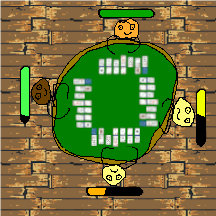
\includegraphics[width=\linewidth]{solitairebr1.png}
\caption{A game of solitaire battle royale.}
\label{Fig:Style1A}
\end{subfigure}\hfill
%
\begin{subfigure}{0.29\linewidth}
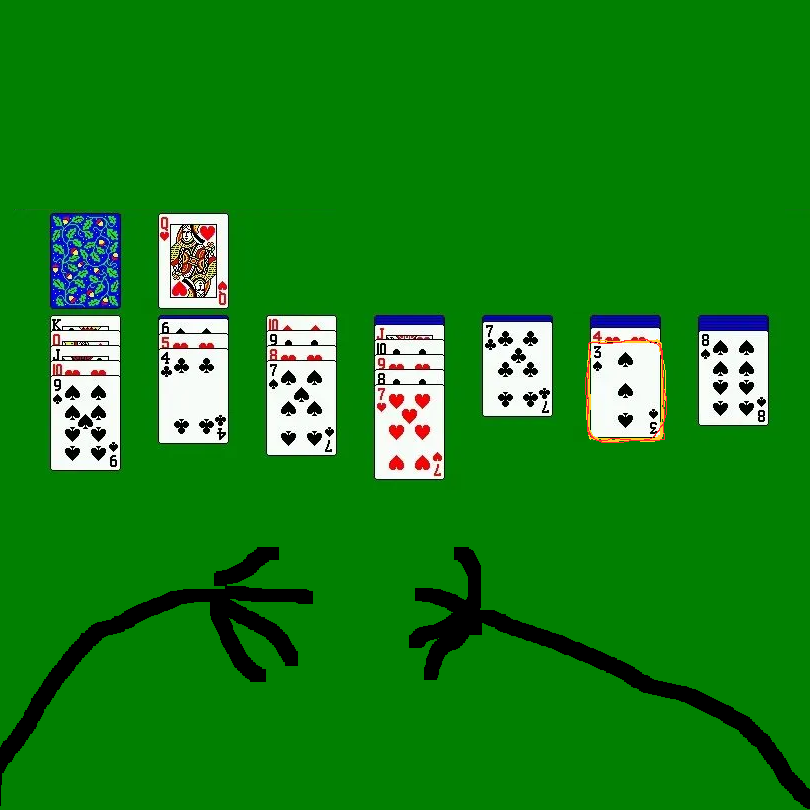
\includegraphics[width=\linewidth]{solitairebr2.png}
\caption{Zoom onto your cards to play more easily.}
\label{Fig:Style1B}
\end{subfigure}\hfill
%
\begin{subfigure}{0.29\linewidth}
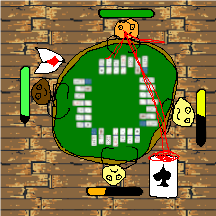
\includegraphics[width=\linewidth]{solitairebr3.png}
\caption{Bottom player is attacking at the top player.}
\label{Fig:Style1C}
\end{subfigure}

\end{figure}

\end{document}
